\documentclass[letter, 12pt]{article}

\usepackage{amsmath,amsthm,amssymb}
\usepackage{fancyhdr}
\usepackage{geometry}
\usepackage{enumerate}
\usepackage{enumitem}
\usepackage{listings}
\usepackage{algorithm}
\usepackage{hyperref}
\usepackage{algorithmic}
\usepackage{eqparbox}
\usepackage{float}
\usepackage{bm}
\usepackage{bbm}
\usepackage{mathtools}
\usepackage{minted}
\usepackage{forest}
\usepackage{cite}

\author{Shengjie Li}
\title{CS 536 : Support Vector Machine Problems}

\pagestyle{fancy}
\fancyhf{} 
\lhead{Shengjie Li \\ netID: sl1560}
\cfoot{\thepage} 
\renewcommand{\headrulewidth}{1pt}
\renewcommand{\headwidth}{\textwidth}
\renewcommand\algorithmiccomment[1]{%
    \hfill\#\ \eqparbox{COMMENT}{#1}%
}
\newlist{subquestion}{enumerate}{1}
\setlist[subquestion, 1]{label = \alph*)}
\DeclareMathOperator*{\argmax}{arg\,max}
\DeclareMathOperator*{\argmin}{arg\,min}

\setlength\parindent{0pt}

% margin adjustment
\addtolength{\textwidth}{1in}
\addtolength{\oddsidemargin}{-0.5in}
\addtolength{\evensidemargin}{-0.5in}
\addtolength{\topmargin}{-.5in}
\addtolength{\textheight}{1.0in}
\setlength\parindent{0cm}

\begin{document}
    \centerline{\textbf{CS 536 : Support Vector Machine Problems}}
    \begin{enumerate}
    	\item{Suppose you had a data set in two dimensions that satisfied the following: the positive class all lay within a certain radius of a point, the negative class all lay outside that radius.}
    	\begin{itemize}
    		\item{Show that under the feature map $ \phi(x_1 , x_2 ) = (1, x_1 , x_2 , x_1 x_2 , x_{1}^2 , x_{2}^2 ) $ (or equivalently, with the kernel $ K(x, y) = (1 + \underline{x}.\underline{y})^2 $ ), a linear separator can always be found in this embedded space, regardless of radius and where the data is centered.}
    		\par{\textbf{Solution:}}
    		\par{From the question we can know that the positive class can be represented in the way of: $ (x_1 - a)^2 + (x_2 - b)^2 \le r $; while the negative class can be $ (x_1 - a)^2 + (x_2 - b)^2 > r $.}
    		\par{Expand the inequality, the positive class would be:}
    			\[(x_1^2 - 2 x_1 a + a^2) + (x_2^2 - 2 x_2 b + b^2) \le r. \]
    		\par{Thus the seperator can be:}
    			\[f(x_1, x_2) = sign(x_1^2 + x_2^2 - 2a x_1 - 2b x_2 + a^2 + b^2 - r). \]
    		\par{If $ f(x_1, x_2) == 1 $, $ (x_1, x_2) $ is in the negative class. If $ f(x_1, x_2) == -1 $, $ (x_1, x_2) $ is in the positive class.}
    		\item{In fact show that if there is an ellipsoidal separator, regardless of center, width, orientation (and dimension!), a separator can be found in the quadratic feature space using this kernel.}
    		\par{\textbf{Solution:}}
    		\par{If there is an ellipsoidal separator, suppose it's unrotated, centered at the origin, of dimension $ d $, then the separator could be:}
    		\[ f(x_1, \dots, x_d) = sign(ax_1^2 + bx_2^2 + \dots + dx_d^2 - 1). \]
    		\par{If $ f(x_1, \dots, x_d) == 1 $, $ (x_1, \dots, x_d) $ is in the negative class. If $ f(x_1, \dots, x_d) == -1 $, $ (x_1, \dots, x_d) $ is in the positive class.}
    		\par{While the quadratic kernel contains a feature map of $ (1, \sqrt{2}x_1, \dots, \sqrt{2}x_d, \sqrt{2}x_1x_2, \dots, x_1^2, \dots, x_d^2)$, it's clear that an unrotated ellipsoidal separator can be found in the quadratic feature space.}
    		\par{For ellipsoidal separators that's not centered at the origin and have some kind of rotation, we can simply see this as the rotation of axes and the shift of the origin, which are just linear transformation on the original equations.}
    		\par{Thus, if there is an ellipsoidal separator, regardless of center, width, orientation and dimension, a separator can be found using this kernel.}
    	\end{itemize}
    	\item{As an extension of the previous problem, suppose that the two dimensional data set satisfied the following: the
    		positive class lay within one of two (disjoint) ellipsoidal regions, and the negative class was everywhere else.
    		Argue that the kernel $ K(x, y) = (1 + \underline{x}.\underline{y})^4 $ will recover a separator.}
    	\par{\textbf{Solution:}}
    	\par{Suppose the first ellipsoidal region $ E_1 $ is $ a_0 (x - x_0)^2 + b_0 (y - y_0)^2 \le r_1 $ and the second one $ E_2 $ is $ a_1 (x - x_1)^2 + b_1 (y - y_1)^2 \le r_2 $, then points of positive class would lie in either $ E_1 $ or $ E_2 $.}
    	\par{Because these two regions are disjoint, if a point $ (x, y) $ lies in $ E_1 $, then $ a_0 (x - x_0)^2 + b_0 (y - y_0)^2 \le r_1 $ and $ a_1 (x - x_1)^2 + b_1 (y - y_1)^2 > r_2 $, which means if a point is in positive class, the results of the equations $ a_0 (x - x_0)^2 + b_0 (y - y_0)^2 - r_1 $ and $ a_1 (x - x_1)^2 + b_1 (y - y_1)^2 - r_2 $ would have different signs.}
    	\par{If a point is in negative class, then the results of the equations $ a_0 (x - x_0)^2 + b_0 (y - y_0)^2 - r_1 $ and $ a_1 (x - x_1)^2 + b_1 (y - y_1)^2 - r_2 $ would have the same sign.}
    	\par{Thus, we can design a classifier: }
    	\begin{align*}
    		f(x, y) &= sign((a_0 (x - x_0)^2 + b_0 (y - y_0)^2 - r_1) * (a_1 (x - x_1)^2 + b_1 (y - y_1)^2 - r_2)) 
    	\end{align*}
    	\par{If $ f(x, y) == 1 $, $ (x, y) $ is in the negative class. If $ f(x, y) == -1 $, $ (x, y) $ is in the positive class.}
    	\par{While $ f(x, y) $ is the multiplication of two polynomials of degree 2 and $ K(x, y) = (1 + \underline{x}.\underline{y})^4 $ is a polynomial kernel of degree 4, we could tell that this kernel will recover a separator.}
    	
    	\item{Suppose that the two dimensional data set is distributed like the following: the positive class lays in a circle centered at some point, the negative class lies in a circular band surrounding it of some radius, and then the additional positive points lie outside that radius. Argue that the kernel $ K(x, y) = (1 + \underline{x}.\underline{y})^4 $ will recover a separator.}
    	\par{\textbf{Solution:}}
    	\par{The positive class would be in $ (x - a)^2 + (y - b)^2 \le r_1 $ or $ (x - a)^2 + (y - b)^2 \ge r_2 $ while the negative class would be in $ r_1 < (x - a)^2 + (y - b)^2 < r_2 $.}
    	\par{If a point is in positive class, then the signs of equations $ (x - a)^2 + (y - b)^2 - r_1 $ and $ (x - a)^2 + (y - b)^2 - r_2 $ would be the same. If a point is in negative class, the signs of equations $ (x - a)^2 + (y - b)^2 - r_1 $ and $ (x - a)^2 + (y - b)^2 - r_2 $ would be different.}
    	\par{Thus, we can use $ f(x, y) = sign(((x - a)^2 + (y - b)^2 - r_1) * ((x - a)^2 + (y - b)^2 - r_2) $ as the separator. If $ f(x, y) == 1 $, $ (x, y) $ is in the positive class. If $ f(x, y) == -1 $, $ (x, y) $ is in the negative class.}
    	\par{Notice that the separator depends on the sign of the multiplication of two polynomials of degree 2, thus the 4-degree polynomial kernel $ K(x, y) = (1 + \underline{x}.\underline{y})^4 $ will recover this separator.}
    	
    	\item{Consider the XOR data (located at $ (\pm1, \pm1) $). Express the dual SVM problem and show that a separator can be found using
    		\begin{itemize}
    			\item{$ K(x, y) = (1 + \underline{x}.\underline{y}) 2 $}
    			\item{$ K(x, y) = exp(-||x - y||^2 ). $}
    		\end{itemize}
    		For each, determine the regions of $ (x_1 , x_2 ) $ space where points will be classified as positive or negative. Given
    		that each produces a distinct separator, how might you decide which of the two was preferred?
    	}
    	\par{The data is:}
    	$ (\underline{x}, y) = 
    	\begin{cases}
    	((-1, -1), -1) \\
    	((-1, +1), 1) \\
    	((+1, -1), 1) \\
    	((+1, +1), -1)
    	\end{cases} $
    	\par{The dual SVM is:}
    	\begin{align*}
    		&\max_{\underline{\alpha}} \sum_{i=1}^{m} \alpha_i - \frac{1}{2} \sum_{i=1}^{m} \sum_{j=1}^{m} \alpha_i y^i K(x^i, x^j) y^j \alpha_j \\
    		&
    		\begin{aligned}
	    		(s.t.) \sum_{i=1}^{m} \alpha_i y^i &= 0 \\
	    		\forall i: \alpha_i &\ge 0.
    		\end{aligned}
    	\end{align*}
    	\par{Denote $ K_{i, j} $ as $ K(x^i, x^j) $, we get:}
    	\begin{align*}
    	&\max_{\alpha_1, \alpha_2, \alpha_3, \alpha_4} [\alpha_1 + \alpha_2 + \alpha_3 + \alpha_4] - \frac{1}{2} [
    	\begin{aligned}[t]
    	&\alpha_1^2 K_{1,1} - 2\alpha_1 \alpha_2 K_{1,2} - 2\alpha_1 \alpha_3 K_{1,3} + 2\alpha_1 \alpha_4 K_{1,4} \\
    	& + \alpha_2^2 K_{2,2} + 2\alpha_2 \alpha_3 K_{2,3} - 2\alpha_2 \alpha_4 K_{2,4} \\
    	& + \alpha_3^2 K_{3,3} - 2\alpha_3 \alpha_4 K_{3,4} \\
    	& + \alpha_4^2 K_{4,4} ] \\
    	\end{aligned} \\
    	&
    	\begin{aligned}
    	(s.t.) -\alpha_1 + \alpha_2 + \alpha_3 -\alpha_4 &= 0 \\
    	\alpha_1, \alpha_2, \alpha_3, \alpha_4 &\ge 0.
    	\end{aligned}
    	\end{align*}
    	\begin{itemize}
    		\item{$ K(x, y) = (1 + \underline{x}.\underline{y})^ 2 $}
    		\par{}
    		$ K = \begin{bmatrix}
    		9 & 1 & 1 & 1 \\
    		1 & 9 & 1 & 1 \\
    		1 & 1 & 9 & 1 \\
    		1 & 1 & 1 & 9 \\
    		\end{bmatrix} $
    		\par{The problem becomes:}
    		\begin{align*}
    		&\max_{\alpha_1, \alpha_2, \alpha_3, \alpha_4} [\alpha_1 + \alpha_2 + \alpha_3 + \alpha_4] - \frac{1}{2} [
    		\begin{aligned}[t]
    		&9 \alpha_1^2 - 2\alpha_1 \alpha_2 - 2\alpha_1 \alpha_3 + 2\alpha_1 \alpha_4 \\
    		& + 9 \alpha_2^2 + 2\alpha_2 \alpha_3 - 2\alpha_2 \alpha_4 \\
    		& + 9 \alpha_3^2 - 2\alpha_3 \alpha_4 \\
    		& + 9 \alpha_4^2 ] \\
    		\end{aligned} \\
    		&
    		\begin{aligned}
    		(s.t.) \alpha_1 + \alpha_4 &= \alpha_2 + \alpha_3 \\
    		\alpha_1, \alpha_2, \alpha_3, \alpha_4 &\ge 0.
    		\end{aligned}
    		\end{align*}
    		\par{After taking partial derivatives and making them 0, we get:}
    		\begin{align*}
    			9 \alpha_1 - \alpha_2 - \alpha_3 + \alpha_4 &= 1 \\
    			-\alpha_1 + 9 \alpha_2 + \alpha_3 - \alpha_4 &= 1 \\
    			- \alpha_1 + \alpha_2 + 9 \alpha_3 - \alpha_4 &= 1 \\
    			\alpha_1 - \alpha_2 - \alpha_3 + 9 \alpha_4 &= 1 .
    		\end{align*}
    		\par{Thus, $ \alpha_1 = \alpha_2 = \alpha_3 = \alpha_4 = 0.25 $.}
    		\par{$ \underline{w}.\underline{x} = \sum_{i=1}^m \alpha_i y^i K(\underline{x^i}, \underline{x}) = \frac{1}{4}(-K(\underline{x}^1, \underline{x}) + K(\underline{x}^2, \underline{x}) + K(\underline{x}^3, \underline{x}) - K(\underline{x}^4, \underline{x}))$.}
    		\par{Choosing $ \underline{x}^1 $ as the support vector, we get the bias value:}
    		\[ b = y^1 - \underline{w}.\underline{x}^1 = -1 \]
    		\par{The classifier is:}
    		\[ f(x) = sign(\frac{1}{4}(-K(\underline{x}^1, \underline{x}) + K(\underline{x}^2, \underline{x}) + K(\underline{x}^3, \underline{x}) - K(\underline{x}^4, \underline{x})) - 1) \]
    		
    		\item{$ K(x, y) = exp(-||x - y||^2 ). $}
    		\par{}
    		$ K = \begin{bmatrix}
    		e^{0} & e^{-4} & e^{-4} & e^{-8} \\
    		e^{-4} & e^{0} & e^{-8} & e^{-4} \\
    		e^{-4} & e^{-8} & e^{0} & e^{-4} \\
    		e^{-8} & e^{-4} & e^{-4} & e^{0} \\
    		\end{bmatrix} $
    		\par{The problem becomes:}
    		\begin{align*}
    		&\max_{\alpha_1, \alpha_2, \alpha_3, \alpha_4} [\alpha_1 + \alpha_2 + \alpha_3 + \alpha_4] - \frac{1}{2} [
    		\begin{aligned}[t]
    		& \alpha_1^2 - 2\alpha_1 \alpha_2 e^{-4} - 2\alpha_1 \alpha_3 e^{-4} + 2\alpha_1 \alpha_4 e^{-8} \\
    		& +  \alpha_2^2 + 2\alpha_2 \alpha_3 e^{-8} - 2\alpha_2 \alpha_4 e^{-4} \\
    		& +  \alpha_3^2 - 2\alpha_3 \alpha_4 e^{-4} \\
    		& +  \alpha_4^2 ] \\
    		\end{aligned} \\
    		&
    		\begin{aligned}
    		(s.t.) \alpha_1 + \alpha_4 &= \alpha_2 + \alpha_3 \\
    		\alpha_1, \alpha_2, \alpha_3, \alpha_4 &\ge 0.
    		\end{aligned}
    		\end{align*}
    		\par{After taking partial derivatives and making them 0, we get:}
    		\begin{align*}
    		 \alpha_1 - \alpha_2 e^{-4} - \alpha_3 e^{-4} + \alpha_4 e^{-8} &= 1 \\
    		-\alpha_1 e^{-4} +  \alpha_2 + \alpha_3 e^{-8} - \alpha_4 e^{-4} &= 1 \\
    		- \alpha_1 e^{-4} + \alpha_2 e^{-8} +  \alpha_3 - \alpha_4 e^{-4} &= 1 \\
    		\alpha_1 e^{-8} - \alpha_2 e^{-4} - \alpha_3 e^{-4} +  \alpha_4 &= 1 .
    		\end{align*}
    		\par{Thus, $ \alpha_1 = \alpha_2 = \alpha_3 = \alpha_4 = \frac{e^8}{(e^4 - 1)^2} $.}
    		\par{$ \underline{w}.\underline{x} = \sum_{i=1}^m \alpha_i y^i K(\underline{x^i}, \underline{x}) =  \frac{e^8}{(e^4 - 1)^2}(-K(\underline{x}^1, \underline{x}) + K(\underline{x}^2, \underline{x}) + K(\underline{x}^3, \underline{x}) - K(\underline{x}^4, \underline{x}))$.}
    		\par{Choosing $ \underline{x}^1 $ as the support vector, we get the bias value:}
    		\[ b = y^1 - \underline{w}.\underline{x}^1 \approx -0.075326 \]
    		\par{The classifier is:}
    		\[ f(x) = sign(\frac{e^8}{(e^4 - 1)^2}(-K(\underline{x}^1, \underline{x}) + K(\underline{x}^2, \underline{x}) + K(\underline{x}^3, \underline{x}) - K(\underline{x}^4, \underline{x})) -0.075326) \]
    	\end{itemize}
    	\par{The regions for these two kernels are:}
    	\begin{figure}[H]
    		\begin{minipage}[b]{.49\textwidth}
    			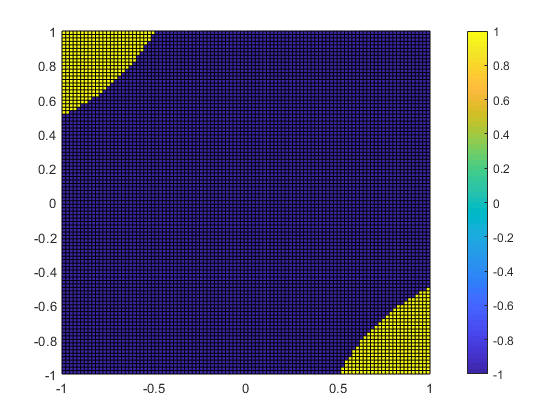
\includegraphics[width=\textwidth]{fig1.png}
    			\caption{$ K(x, y) = (1 + \underline{x}.\underline{y})^ 2 $}
    			\label{fig1}
    		\end{minipage}
	    	\begin{minipage}[b]{.49\textwidth}
		    	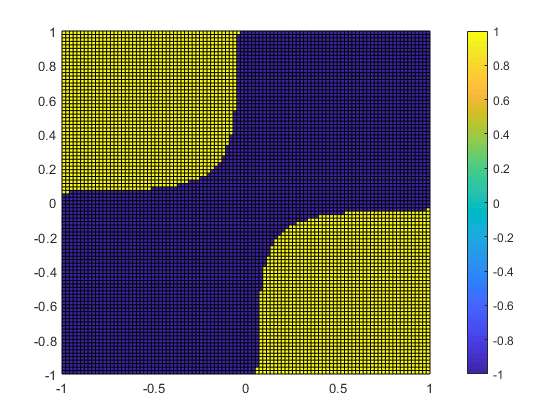
\includegraphics[width=\textwidth]{fig2.png}
		    	\caption{$ K(x, y) = exp(-||x - y||^2 ). $}
		    	\label{fig2}
		    \end{minipage}
    		\centering
    	\end{figure}
    	\par{By calculating the margin of two classifiers, we would know which classifier is better.}
    	\par{Also, from the Fig \ref{fig1} and Fig \ref{fig2}, we can tell SVM with $ K(x, y) = exp(-||x - y||^2 ). $ has a better margin.}
    \end{enumerate}
\end{document}
